\graphicspath{{./figs/Chp-PWGaBP/}}

%%Fakesection Acronym reset
\glsreset{acr:pwgabp}
\glsreset{acr:sdd}
\glsreset{acr:dpcg}
\glsreset{acr:sus}
\glsreset{acr:pus}
\glsreset{acr:hus}
\glsreset{acr:pwgm}
\glsreset{acr:rcm}

\chapter{Schedule Implementations for Gaussian Belief Propagation}


\label{chp:PW-GaBP}
In this chapter, we introduce implementation-oriented scheduling schemes for the \gls{acr:pwgabp} solver aimed at large sparse linear systems obtained from \gls{acr:fem} applications.
We analyze different message scheduling schemes used to enhance implementations, CPU time, and parallel executions.
Our empirical experiments show that \gls{acr:pwgabp} when used with \gls{acr:sdd} matrices can potentially result in execution-times that are competitive with the widely used \gls{acr:dpcg} solver.


We present empirical results of the \gls{acr:sus} of the \gls{acr:pwgabp} solver.
Compared with the \gls{acr:dpcg} solver, the \gls{acr:sus} demonstrates considerable reduction in iteration count for large sparse \gls{acr:sdd} linear systems.
Next, we present the \gls{acr:hus} for the \gls{acr:pwgabp}.
The \gls{acr:hus} algorithm uses an appropriate mix of sequential and parallel message updates.
The parallel implementations of the \gls{acr:hus} demonstrates that, the \gls{acr:hus} facilitates efficient parallel execution while demonstrating faster convergence rates typical of \gls{acr:pwgabp} using \gls{acr:sus}.


\section{Introduction}

In this work, we present various scheduling implementations for the \gls{acr:pwgabp} to solve large sparse linear systems arising from the \gls{acr:fem} problem.
We, therefore, assume that the sparse matrix $A$ for the underlying \gls{acr:fem} problem is already assembled by other \gls{acr:fem} software such as \libName{GetFEM} \cite{bib:getfem}.
The computational efficiency of a \gls{acr:pwgabp} implementation will depend largely on two factors: the data-structure used to store the nodes' connectivities as provided by the \gls{acr:pwgm} along with communicated messages, and the message transfer medium such as the memory bandwidth for shared-memory architectures or the network bandwidth for CPU-clusters.
From an implementation perspective, three distinct stages can be designated for the nodal message update process of the \gls{acr:pwgabp} algorithm.
First, the node receives messages from sparse connections.
Second, the node performs local computations using the received messages.
Last, the node responds with new messages on the same sparse connections.
For CPU implementations, the choice of the data-structure required to store the messages will have a critical impact on the overall performance of the \gls{acr:pwgabp} algorithm due to the predominant message access time, data-locality and vectorization of computational loops.
However, sparse matrices arising from typical \gls{acr:fem} applications can exhibit a banded sparsity structure when proper reordering algorithms are used, which can be exploited to increase the parallel \gls{acr:pwgabp} performance.


\gls{acr:pwgabp} message updates are performed subject to a particular schedule.
Two basic scheduling schemes common in general \gls{acr:bp} algorithms are the \gls{acr:sus}, and the \gls{acr:pus}, also known as flooding.  
In the \gls{acr:sus}, nodes are processed in sequence according to a particular ordering; while messages are propagated sequentially to receiving nodes in the same iteration.  
Hence, the \gls{acr:sus} scheme provides little opportunity for parallel processing.
The \gls{acr:pus}, on the other hand, facilitates fully concurrent execution of the nodes; however, the \gls{acr:pus} requires a considerably larger number of iterations compared to \gls{acr:sus}.
Specifically, the empirical analysis in \cite{bib:Elidan06ResidualBP,bib:Bertsekas1983DACFP} and other references within, indicates that the convergence rate of the \gls{acr:sus} is upper-bounded by the convergence rate of the \gls{acr:pus}.
The work in \cite{bib:Elidan06ResidualBP,bib:gonzalez2009residual} also uses an informative based scheduling scheme which is used to accelerate convergence; in addition this scheme, in certain cases, can achieve convergence for models where basic \gls{acr:bp} fails.  
However, this work mainly uses discrete-domain probabilistic models of relatively small size compared to the large models resulting from \gls{acr:fem} applications where the number of real-domain variables range in the order of millions or billions.
Therefore, we believe that the \gls{acr:bp} scheduling for \gls{acr:fem} problems should be treated as an implementation feature to enhance parallelism of the algorithm rather than to improve the convergence rate.
The convergence rate, on the other hand, can more efficiently be treated using a specialized multigrid scheme for \gls{acr:bp} as we later show in \chpRef{chp:FMGaBP}.


This chapter is organized as follows.
In \secRef{sec:sus} we present the \gls{acr:sus} implementation of the \gls{acr:pwgabp} algorithm. 
In \secRef{sec:pus} we present the \gls{acr:pus} implementation.
In \secRef{sec:hus} we present the \gls{acr:hus} implementation.
Finally, in \secRef{sec:pwgabpRes} we conclude with performance results.

\section{Sequential Update PW-GaBP}
\label{sec:sus}


In \algRef{alg:seq_gabp} we present a particular implementation of \gls{acr:pwgabp} which makes efficient use of contiguous data-structures such as queues or stacks to store and retrieve messages.
This particular implementation uses the \gls{acr:sus} scheme.
Using simple data-structures such as stacks or queues results in constant-time per message access complexity for retrieval and insertion, reducing the algorithm's overall message processing complexity per iteration to $\bigo{\gls{acr:nnz}}$, where \gls{acr:nnz} is the number of non-zeros in $A$.
Using such data-structures is facilitated by adding the source node pointer ($n_i$) and the edge element parameter ($A_{i,j}$) to the message.
Stacks are used in all our implementations; however, queues can also be used instead of stacks without much impact on the algorithm's performance.  
It is important to note that this implementation results in a fixed increase in the memory requirement per each message.  
However, since this fixed increase in the message size is independent of the problem's overall size $N$, where $N$ is the number of variables, the algorithm's overall memory complexity scales linearly with $N$ as expected for sparse problems.


In the \gls{acr:sus}, the nodes need to be processed according to a particular order.
In addition, the initialization stage is critical for the correct operation of the algorithm.
As shown in lines 2 to 6, a unique nodal ordering ($\kappa$) needs to be defined.
The nodes are also initialized with zero messages subject to the ordering $\kappa$.
In this algorithm, a single processing node is assumed that has access to the full data-structure of $A$.
While the \gls{acr:sus} is not practical for parallel implementations, its study provides a hypothetical lower bound on the iteration count of the \gls{acr:pwgabp} solver when used with linear systems resulting from \gls{acr:fem} applications.

% Sequential version of \gls{acr:pwgabp} Algorithm
\begin{algorithm}[h]
	\centering
	\begin{algorithmic}[1]

		\STATE \textit{Initialize: }

		\STATE Define node ordering: $ \kappa $

		\FOR{each edge $A(i,j)$}

		\IF{$ n_i <_{\kappa} n_j$}
		\STATE $n_i.\OpN{push}(n_j.\OpN{pointer},A_{ij}, P_{ji} = 0, \mu_{ji} = 0) $
	\ENDIF

\ENDFOR

\STATE \textit{Compute: }
\REPEAT[iterations]
\FOR{ each node $n_i \in \kappa $}
\STATE $ P_{agg} = A_{ii} + \sum_{k} P_{ki}$
\STATE $ \mu_{agg} = b_{i} + \sum_{k} \mu_{ki}$

\FOR{ each received message $n_j \rightarrow n_i$ }
\STATE $\mu_{ij} = -A_{ij} (P_{agg} - P_{ji})^{-1} (\mu_{agg} - \mu_{ji}) $
\STATE $P_{ij} = -A_{ij}^2 (P_{agg} - P_{ji})^{-1} $
\STATE $n_i.\text{pop\_message}$
\STATE $n_j.\OpN{push}(n_i.\OpN{pointer},A_{ij}, P_{ij}, \mu_{ij})$
\ENDFOR
\STATE $\overline{x_i} = \mu_{agg} P_{agg}^{-1}$

\ENDFOR
\UNTIL{\textit{convergence:} all $\overline{x_i}$ converged}
\STATE \textit{Output:} $\overline{x_{i}}$
\end{algorithmic}

\caption{The sequential update \acrshort{acr:pwgabp} implementation-oriented algorithm.}
\label{alg:seq_gabp}
\end{algorithm}

\section{Parallel Update PW-GaBP}
\label{sec:pus}

The \gls{acr:pus} version of the \gls{acr:pwgabp} algorithm is shown in \algRef{alg:par_gabp}.
This algorithm uses arrays of local static memory to store the node's edge messages.
The local memory array provides constant time access on shared-memory machines by assigning a specific memory location to each destination node.
To facilitate concurrent execution of all nodes, each node contains two message arrays, a current-message array that stores messages received in the previous iteration and is used to compute the new messages in the current iteration, and a new-message array that is used to store the new messages being received from the edge nodes in the current iteration.
Alternately, coloring schemes can be used to resolve memory collisions as proposed later in \chpRef{chp:FMGaBP}.
At the beginning of each iteration, each node collects its edge messages into the new message buffer then swaps the current and the new message buffer pointers.
Constant-time access data-structures such as queues and stacks can be used instead of static memory arrays.
Also, there is no need to define any node ordering as the case in the \gls{acr:sus} algorithm.
Since the number of processing elements in computing environments is typically much less than the number of nodes, the \gls{acr:pus} algorithm may not be practical for implementations targeted for large linear systems; nonetheless, the algorithm has conceptual importance for approximating the upper bound on the parallel iteration count.

% Parallel version of \gls{acr:pwgabp} Algorithm
\begin{algorithm}[h]
	\centering
	\begin{algorithmic}[1]
		\STATE \textit{Initialize:}
		\FOR{each edge $A(i,j)$}
		\STATE $n_i.\OpN{send}(n_j.\OpN{pointer},A_{ij}, P_{ji} = 0, \mu_{ji} = 0)$
		\AlgENDFOR
		\STATE \textit{Compute: }
		\REPEAT[iterations]
		\FOR{each node $n_i$ }
		\STATE $n_i.\OpN{swap\_pointers}(\OpN{currMessArray},\OpN{newMessArray})$
		\AlgENDFOR
		\FOR[concurrent execution]{ each node $n_i$ }
		\STATE Using the current-message buffers
		\STATE $ P_{agg} = A_{ii} + \sum_k P_{ki}$
		\STATE $ \mu_{agg} = b_{i} + \sum_k \mu_{ki}$
		\FOR{each received message $n_j \rightarrow n_i$ }
		\STATE $\mu_{ij} = -A_{ij} (P_{agg} - P_{ji})^{-1} (\mu_{agg} - \mu_{ji}) $
		\STATE $P_{ij} = -A_{ij}^2 (P_{agg} - P_{ji})^{-1} $
		%\STATE $n_i.\OpN{pop\_message}$
		\STATE $n_j.\OpN{send}(n_i.\OpN{pointer},A_{ij}, P_{ij}, \mu_{ij})$
		\AlgENDFOR
		\STATE $\overline{x_i} = \mu_{agg} P_{agg}^{-1}$
		\AlgENDFOR
		\UNTIL{\textit{convergence:} all $\overline{x_i}$ converged}
		\STATE \textit{Output:} $\overline{x_{i}}$
	\end{algorithmic}
	\caption{The parallel update \acrshort{acr:pwgabp} implementation-oriented algorithm.}
	\label{alg:par_gabp}
\end{algorithm}


\section{Hybrid Update PW-GaBP}
\label{sec:hus}

Since in typical parallel computing environments the number of processing elements is limited, a degree of sequential processing will have to be performed for large problems.
Our implementation-oriented \gls{acr:hus} algorithm, shown in \algRef{alg:hyb_gabp}, takes advantage of this imposed sequentiality to propagate faster message information, which reduces the \gls{acr:pwgabp} iteration count while exploiting parallelism in both single-node and multi-node \glspl{acr:hpc}.


By creating a partitioning scheme of relatively adjacent nodes, where each partition is assigned to a processing element to be executed in parallel, updates between nodes in different partitions can be performed using the \gls{acr:pus} algorithm, while updates between nodes in the same partition can be performed using the \gls{acr:sus} algorithm.
This flexibility allows the \gls{acr:hus} algorithm to easily implement different sequential-parallel scheduling variations by varying the partition boundaries and the node ordering within each partition.
That is, by choosing a partitioning and an ordering scheme that exploits node locality in terms of connectivity.
The number of iterations increase due to parallel message updates can be expected to be considerably reduced, which will be demonstrated later in our results.

% Hybrid version of \gls{acr:pwgabp} Algorithm
\begin{algorithm}[!t]
	\centering
	\begin{algorithmic}[1]
		\small
		\STATE \textit{Initialize:}
		\STATE Define node partitioning $\zeta $
		\STATE Define node ordering $\kappa$ in each $\zeta$
		\FOR{each edge $A(i,j)$}
		\IF[nodes in the same partition]{$n_i =_\zeta n_j$}
		\IF{$ n_i <_{\kappa} n_j$}
		\STATE $n_i.\OpN{push}(n_j.\OpN{pointer},A_{ij}, P_{ji} = 0, \mu_{ji} = 0) $
		\AlgENDIF
		\ELSE[nodes not in the same partition]
		\STATE $n_i.\OpN{send}(n_j.\OpN{pointer},A_{ij}, P_{ji} = 0, \mu_{ji} = 0)  $
		\AlgENDIF
		\AlgENDFOR
		\STATE \textit{Compute: }
		\REPEAT[iterations]
		\FOR{ each node $n_i$ on partition edge }
		\STATE $n_i.\OpN{swap\_pointers}(\OpN{currMessArray},\OpN{newMessArray})$
		\AlgENDFOR
		\FOR[concurrent execution] { each partition in $\zeta $}
		\FOR[sequential execution]{ each node $n_i \in \kappa$ }
		\STATE $ P_{agg} = A_{ii} + \sum_k P_{ki}$
		\STATE $ \mu_{agg} = b_{i} + \sum_k \mu_{ki}$

		\FOR{ each received message $n_j \rightarrow n_i$ }
		\STATE $\mu_{ij} = -A_{ij} (P_{agg} - P_{ji})^{-1} (\mu_{agg} - \mu_{ji}) $
		\STATE $P_{ij} = -A_{ij}^2 (P_{agg} - P_{ji})^{-1} $
		\IF{$n_j$ in the same partition}
		\STATE $n_i.\OpN{pop\_message}$
		\STATE $n_j.\OpN{push}(n_i.\OpN{pointer},A_{ij}, P_{ij}, \mu_{ij})$
		\ELSE
		\STATE $n_j.\OpN{send}(n_i.\OpN{pointer},A_{ij}, P_{ij}, \mu_{ij})$
		\AlgENDIF
		\AlgENDFOR
		\STATE $\overline{x_i} = \mu_{agg} P_{agg}^{-1}$
		\AlgENDFOR

		\AlgENDFOR
		\UNTIL{\textit{convergence:} all $\overline{x_i}$ converged}
		\STATE \textit{Output:} $\overline{x_{i}}$
	\end{algorithmic}
	\caption{The hybrid update \gls{acr:pwgabp} implementation-oriented algorithm.}
	\label{alg:hyb_gabp}
\end{algorithm}


\section{Results and Discussions}
\label{sec:pwgabpRes}



\subsection{Performance Comparison with D-PCG}


In order to assess the computational speed of the \gls{acr:sus}, we compare it with the \gls{acr:dpcg} algorithm.
All runs are executed on single CPU workstation with Intel Core2 Quad @ 2.8GHz using double-precision computations.
The \gls{acr:dpcg} code was executed on the same CPU and it was obtained from the optimized \libName{GMM++} library \cite{bib:gmm}.
Iterations were stopped when the $l^2$-norm of the residual reached $\epsilon = 10^{-9}$.
The test matrices, shown in \tableRef{tbl:testMatrices}, are obtained from \cite{bib:UFSparseMatrix}, with the exception of the matrix ``Random'' which is generated randomly using the Matlab software \cite{bib:matlab2013}.
The matrix ``thermal2'' results from an unstructured steady-state \gls{acr:fem} application.
The matrices were made diagonally dominant by loading the diagonals with a uniformly distributed positive random number having a standard deviation $\sigma \in [10^{-2},10^3]$, in order to make the matrices conform with the walk-summability criteria \cite{bib:Johnson2006WIAGBP} required for the \gls{acr:pwgabp} convergence.
The plots in \figRef{fig:su} show the performance results of the \gls{acr:pwgabp} solver using the \gls{acr:sus} scheme against the \gls{acr:dpcg} solver.
Iteration reductions, up to 6$\times$, are obtained by the \gls{acr:sus} \gls{acr:pwgabp} algorithm.
Also, the \gls{acr:sus} implementation was able to achieve time speedups for many cases reaching up to 1.8$\times$.
It is worth noting that the obtained time speedup gains do not match the gains from the iteration reductions, which we attribute to the fact that the \libName{GMM++} implementation of the \gls{acr:dpcg} algorithm has more efficient memory bandwidth utilization for sequential execution than our algorithm.
However, the \gls{acr:pwgabp} algorithm is more tailored towards parallel implementations than the \gls{acr:pcg} algorithm.

\begin{table}
	\centering
	\begin{threeparttable}[c]
		\caption{Sparse test matrices.}
		\label{tbl:testMatrices}
		\centering
		%\begin{tabular}{lcccc}
		\begin{tabular}{ >{\centering\arraybackslash}m{.7in}  >{\centering\arraybackslash}m{.7in}  >{\centering\arraybackslash}m{.9in}  >{\centering\arraybackslash}m{.7in}  >{\centering\arraybackslash}m{.7in} }
			\toprule
			\flushleft Category & ecology1 & G3{\_}circuit & thermal2 & random\\
			\midrule
			\flushleft N (nodes) & 1,000,000 & 1,585,478 & 1,228,045 & 1,000,000 \\
			\flushleft $\OpN{nnz} $ & 4,996,000 & 7,660,826 & 8,580,313 & 8,999,976 \\
			\bottomrule
		\end{tabular}
	\end{threeparttable}
\end{table}

%%
\begin{figure}[!t]
	\centerline{
	\subfloat[]{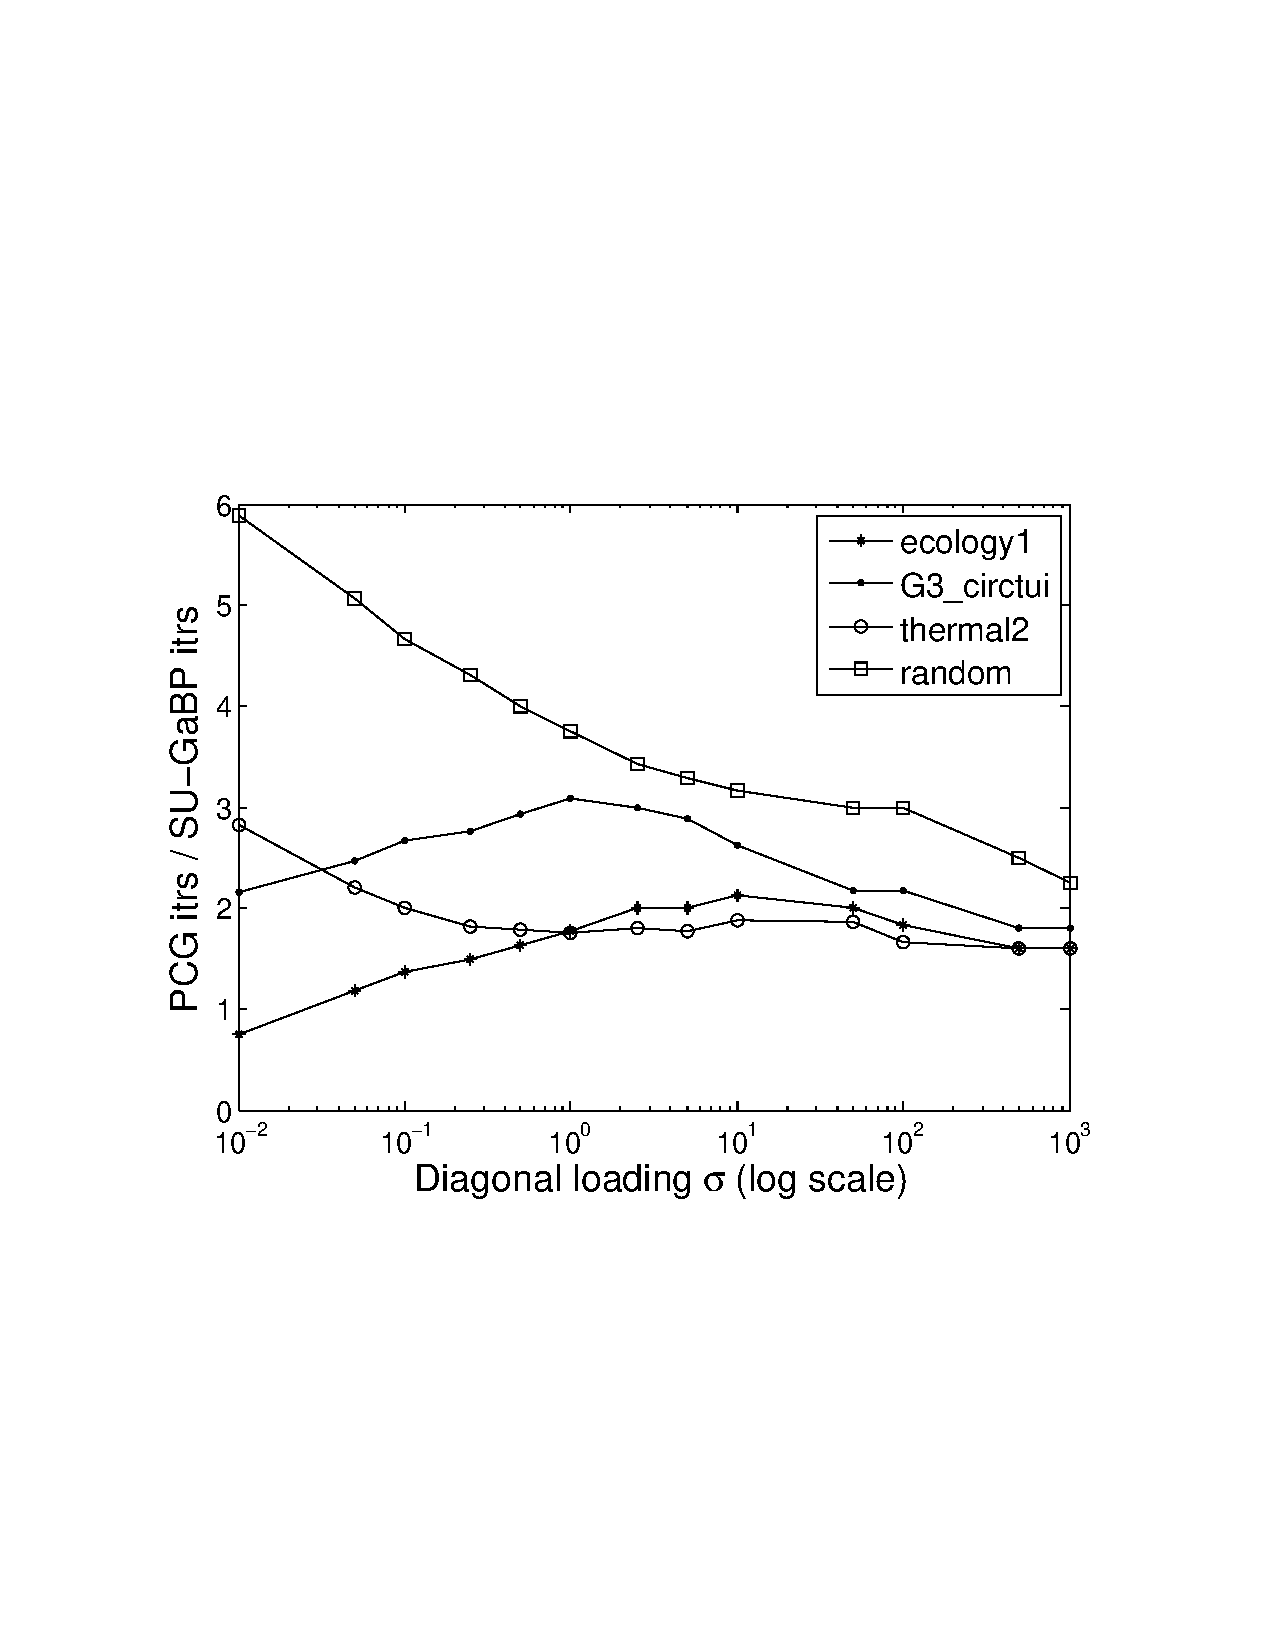
\includegraphics[width=2.8in]{FIG2}}
	\hfill
	\subfloat[]{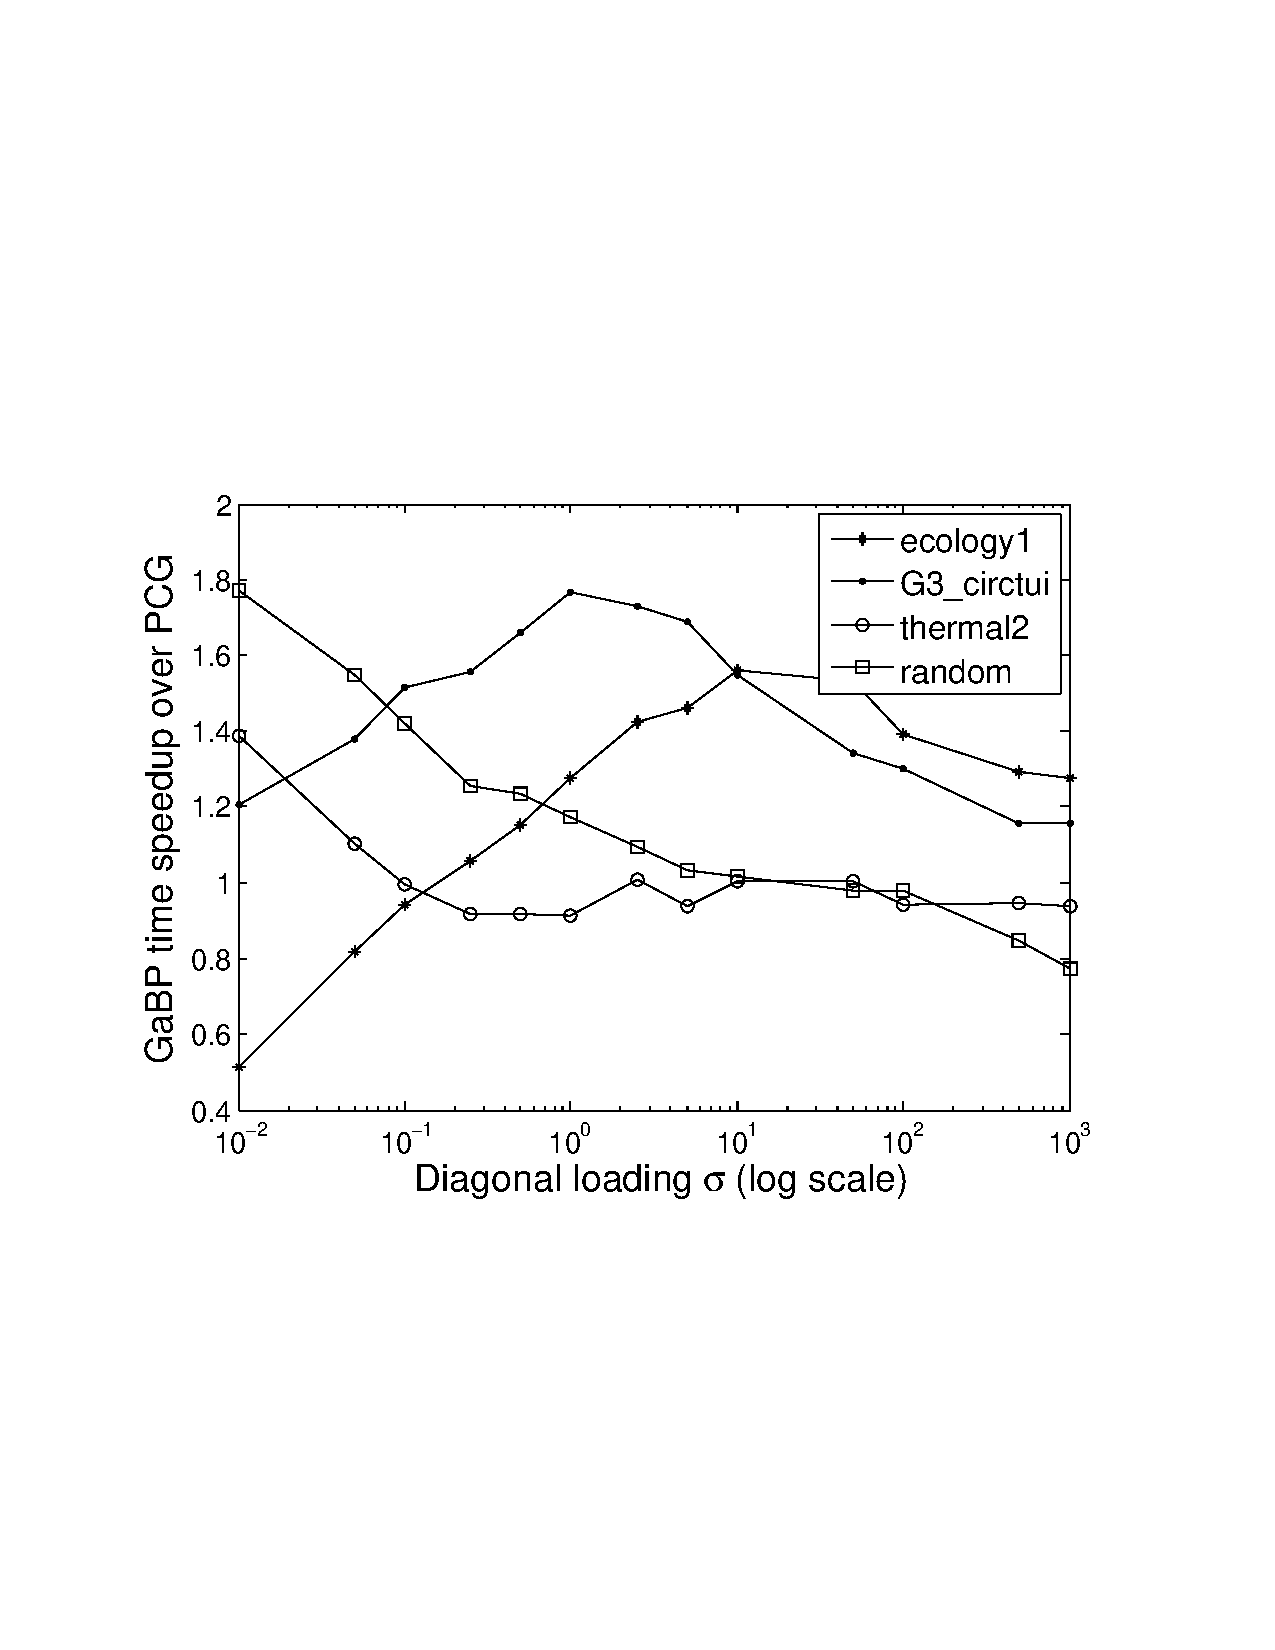
\includegraphics[width=2.8in]{FIG3}}
	}
	\caption[Speedup of the \acrshort{acr:pwgabp} implementation over \acrshort{acr:dpcg}.]{Speedup of the implementation-oriented \gls{acr:pwgabp} using the \gls{acr:sus} scheme. (a) Iteration improvement of \gls{acr:pwgabp} over \gls{acr:dpcg}. (b) \gls{acr:pwgabp} time speedup over \gls{acr:dpcg}.}
	\label{fig:su}
\end{figure}

\subsection{Hybrid-Update Scheduling Performance}

The parallel behavior of the \gls{acr:pwgabp} algorithm using the \gls{acr:hus} implementation was simulated on a single-core CPU.
In order to simulate different partitioning and node ordering, matrix reordering techniques were used.
Two common reordering techniques used here are: the \gls{acr:rcm} \cite{bib:Cuthill1969RTBOSSM}, which reduces the matrix bandwidth; and \gls{acr:amd}, which produces large blocks of zeros \cite{bib:George1989TEOTMDOA}. 
\figRef{fig:hu-gabp} shows the parallel results of our \gls{acr:hus} implementation algorithm on the matrix ``thermal2'' as the number of parallel partitions increases from 1 to 4096.
The \gls{acr:hus} algorithm demonstrates gradual rate of increase in iterations on the original unordered matrix, while ordered matrices using the \gls{acr:rcm} and the \gls{acr:amd} algorithms showed a considerably lower rate of increase.
These results demonstrate the \gls{acr:hus} potential for parallel gains and its ability in exploiting the problem's connectivity structure by maintaining a lower iteration count than the \gls{acr:pus} scheme.
These results also suggest that good speedup gains can be obtained from implementing the \gls{acr:hus} on CPU-clusters and many-core architectures in comparison with leading iterative methods such as the \gls{acr:dpcg} algorithm.

\begin{figure}
	\centerline{
	\subfloat[]{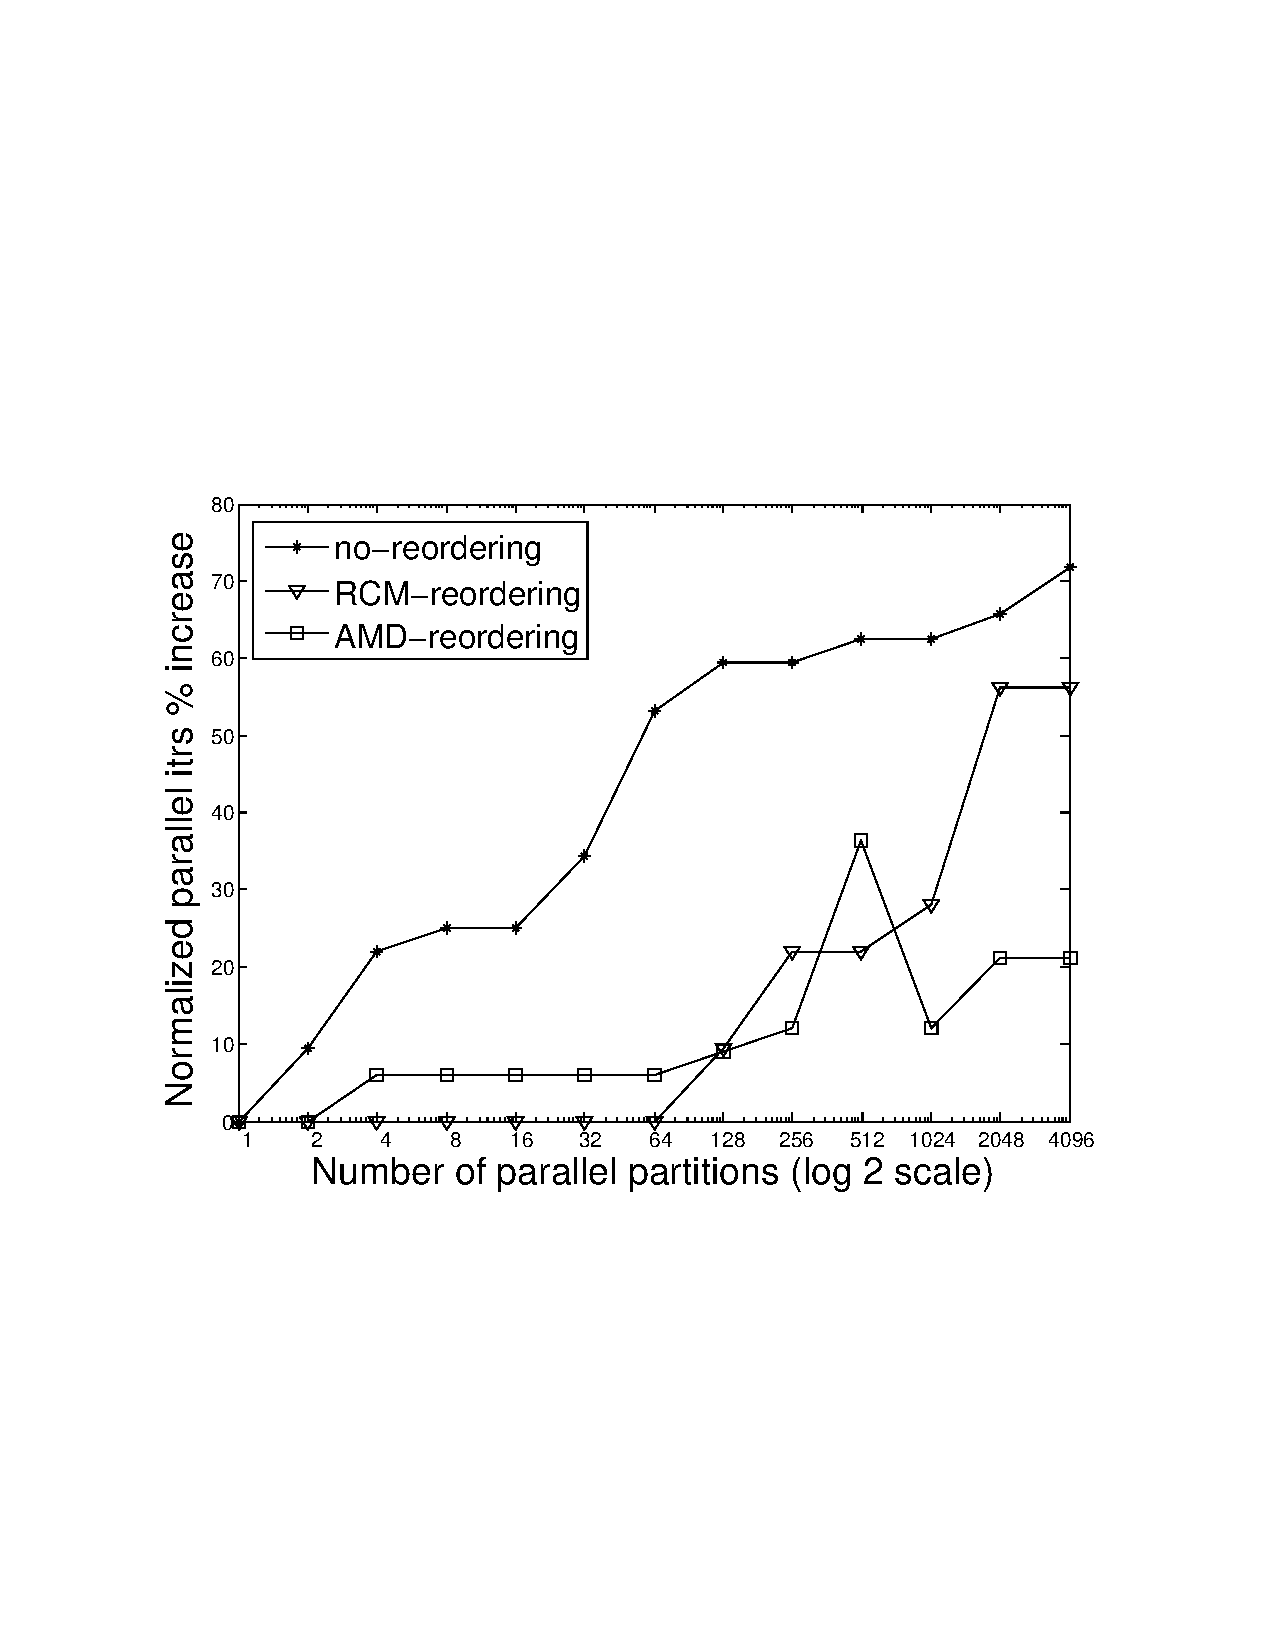
\includegraphics[width=3.0in]{FIG4}}
	}
	\centerline{
	\subfloat[]{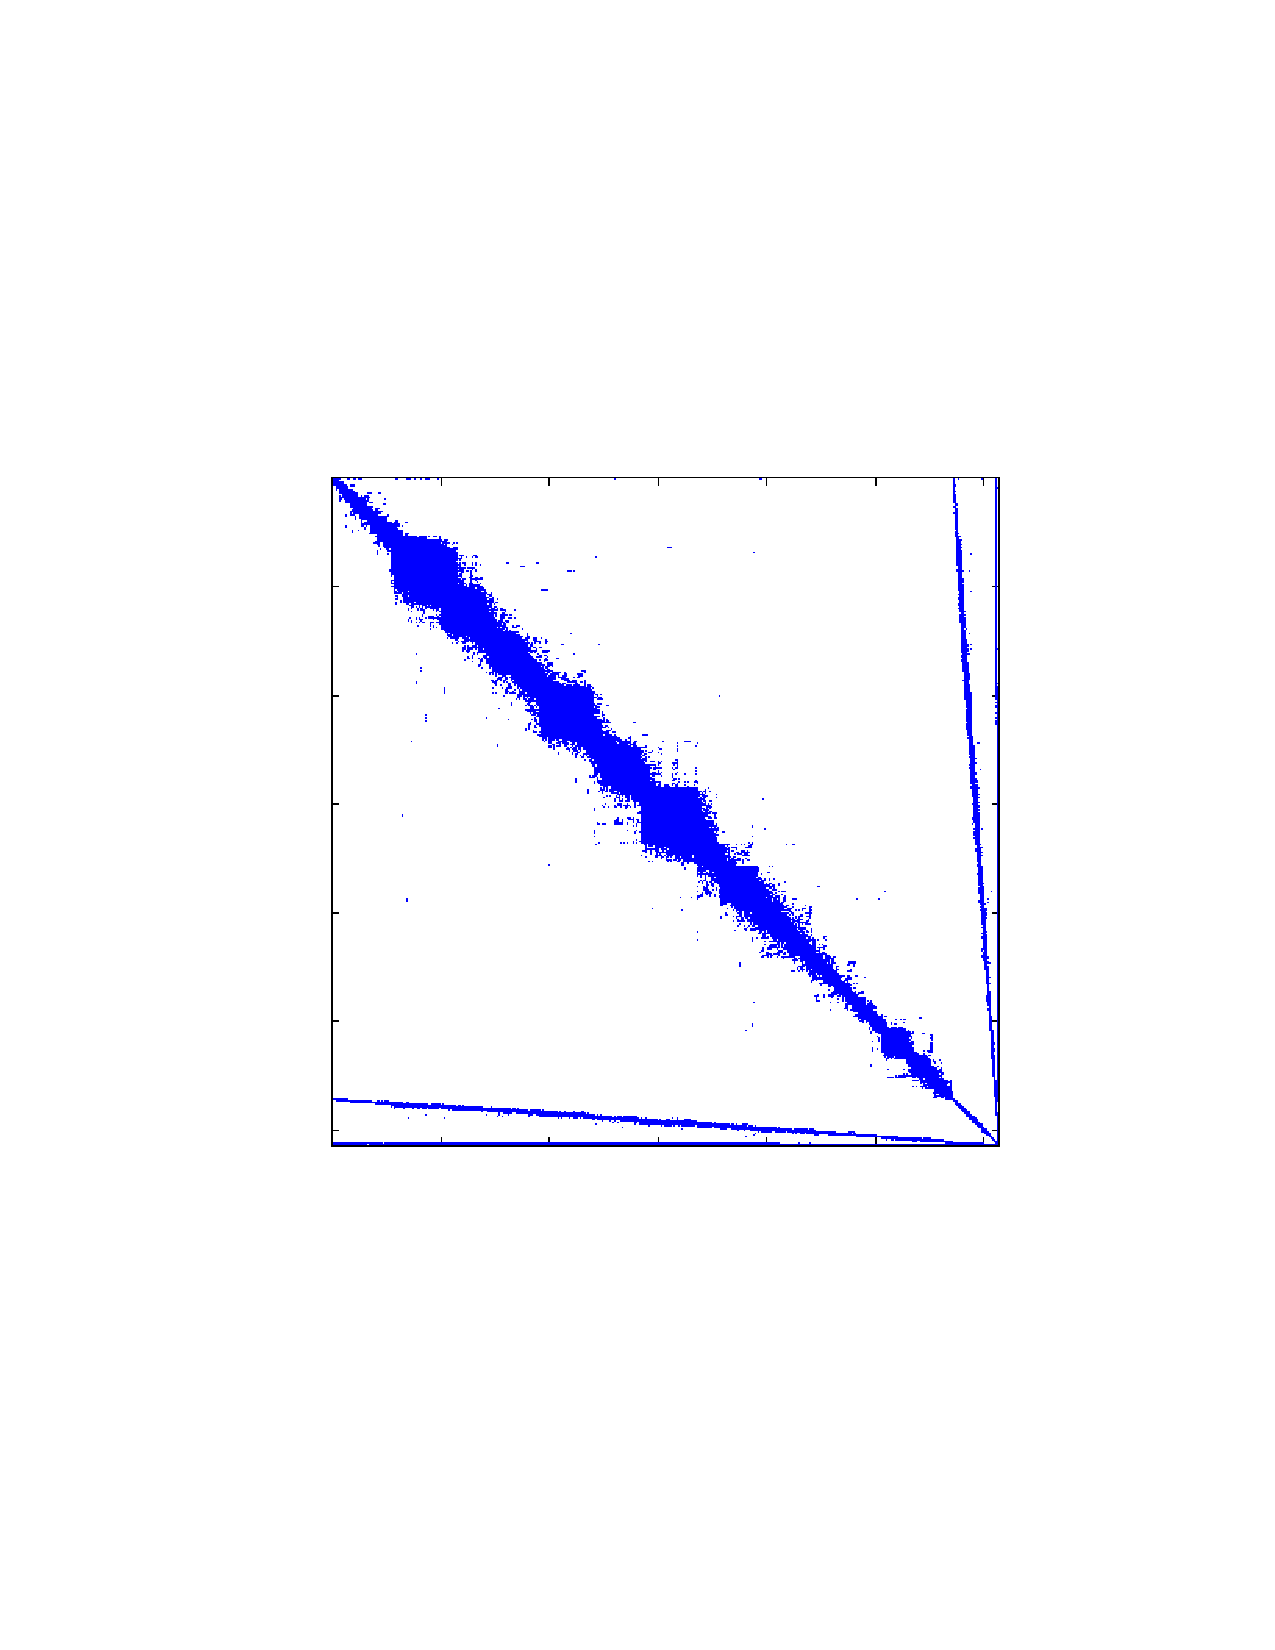
\includegraphics[width=.8in]{FIG5}}
	\hfil
	\subfloat[]{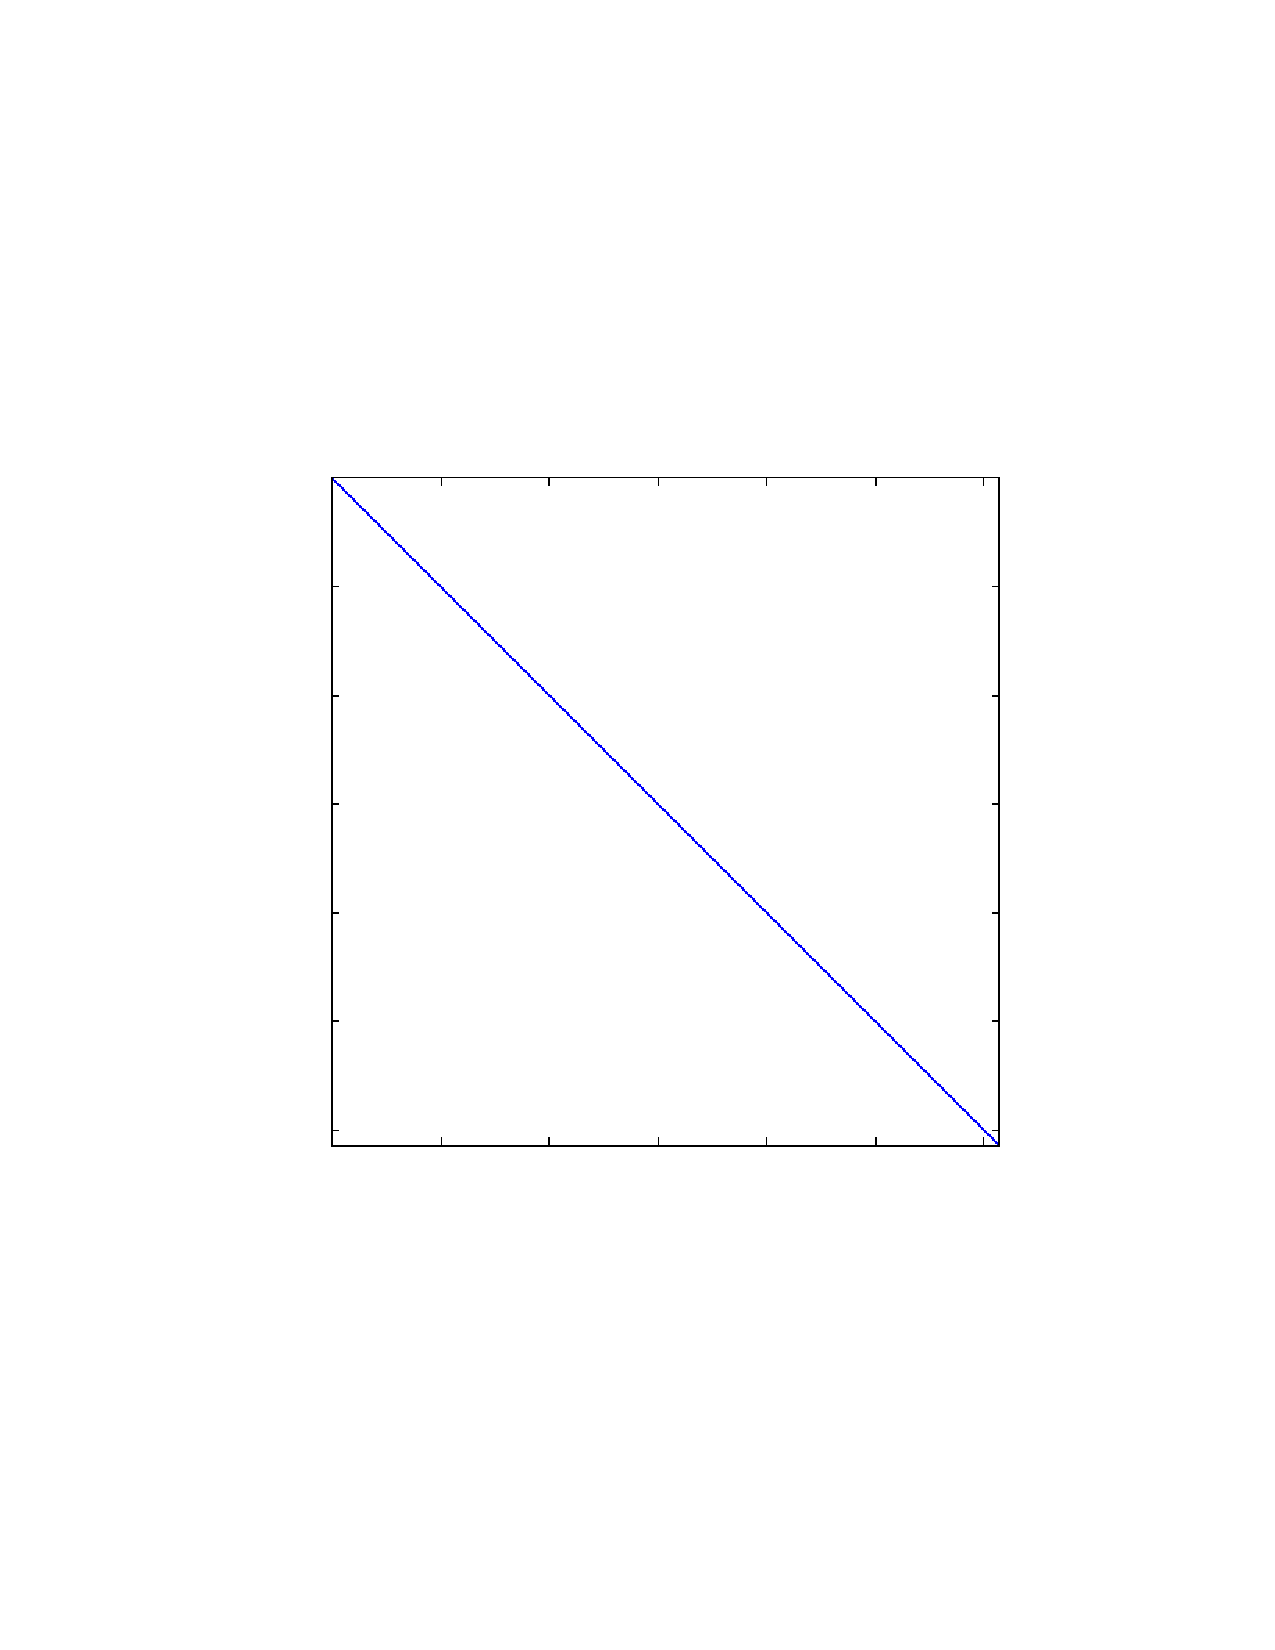
\includegraphics[width=.8in]{FIG6}}
	\hfil
	\subfloat[]{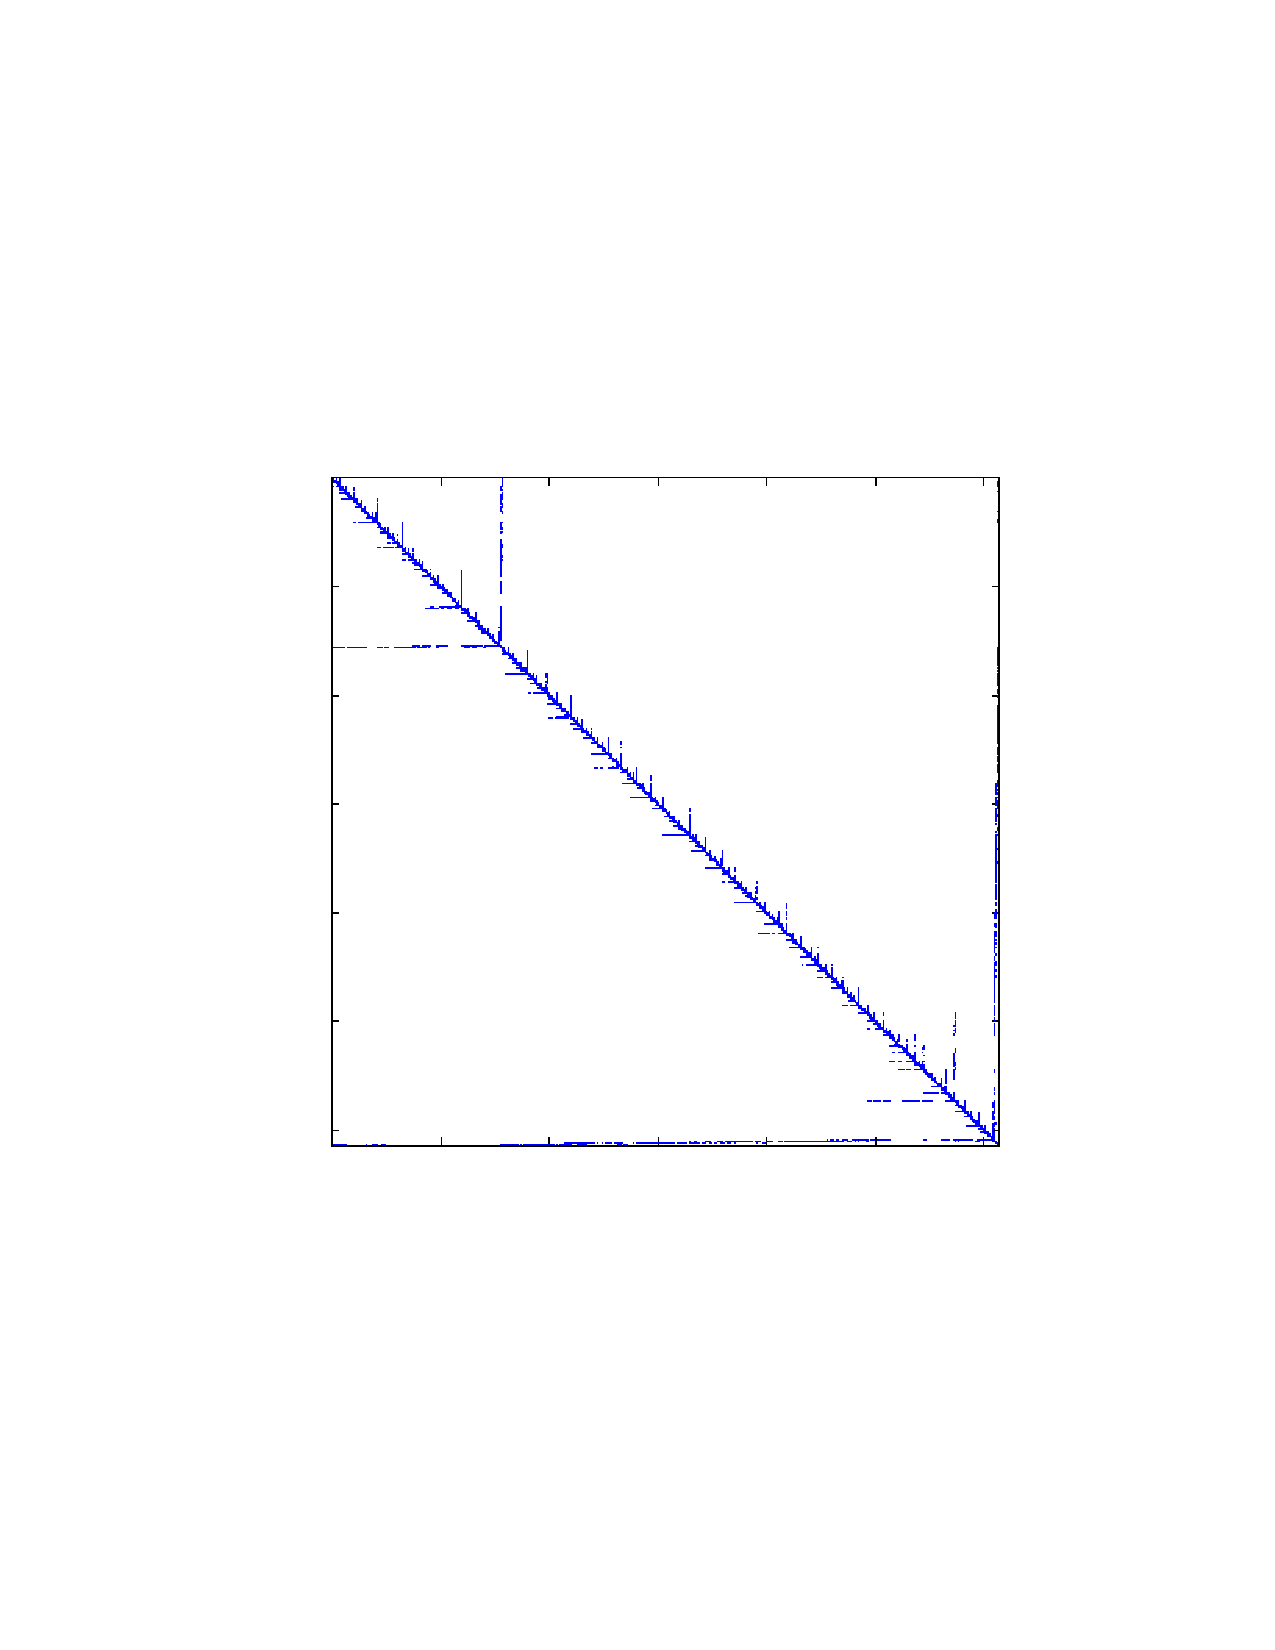
\includegraphics[width=.8in]{FIG7}}
	}
	\caption[The \acrshort{acr:pwgabp} algorithm results using the \acrshort{acr:hus} scheme.]{The \gls{acr:pwgabp} algorithm results using the \gls{acr:hus} scheme for the matrix ``thermal2'. (a) The \gls{acr:hus} parallel iteration increase rate. (b) Sparsity structure of original ''thermal2.`` (c) \gls{acr:rcm} reordered. (d) \gls{acr:amd} reordered.}
	\label{fig:hu-gabp}
\end{figure}


\section{Conclusion}
Implementation-oriented algorithms of \gls{acr:pwgabp} were presented which demonstrated speedups of up 1.8$\times$ over the \gls{acr:dpcg} algorithm.
Also, both improvements in execution time and reduction in iteration count over the \gls{acr:dpcg} solver were demonstrated using the \gls{acr:pwgabp} algorithm with the \gls{acr:sus} scheme.
While the \gls{acr:pwgabp} solver demonstrated an advantage over the \gls{acr:dpcg} solver for \gls{acr:sdd} matrices, the performance for more general \gls{acr:fem} matrices is clearly not competitive against leading solvers such as \gls{acr:icpcg} or multigrid; nonetheless, this study provides valuable insights for the later development and implementation of the \gls{acr:fgabp} and the \gls{acr:fmgabp} algorithms presented in Chapters \ref{chp:FGaBP} and \ref{chp:FMGaBP} which fix the convergence rate issue.
The \gls{acr:hus} algorithm was introduced and its implementation demonstrated enhanced parallel performance for \gls{acr:pwgabp}.
The \gls{acr:hus} algorithm results showed considerable reductions in parallel iterations demonstrating great potential for efficient implementations on CPU-clusters and many-core \gls{acr:hpc} platforms.
